
\chapter{MLExplore.js: A Web Interactive Tool for Exploring High-Dimensional Data}
\label{chapter3}

\graphicspath{{Chapter3/figs/}}

From Chapter \ref{chapter2}, 4 interface elements to be included in an Interactive ML system are stated and Interpretable ML is proposed as a mechanism for complementing the \textbf{model inspection} and \textbf{task overview} elements. This chapter also highlights some relevant works for interacting with and interpreting DR and Clustering models for data analysis. An important focus of the state of the art proposals in Interactive ML is to provide user with the ability for hyper-parameter exploration looking to produce a good representation of embeddings and clusters. The discussion about what is a good representation, being the general problem in unsupervised learning, continues open. In addition, researchers also focus on deriving the most relevant interaction elements for supporting the data exploration. These proposals can be complemented with components for data exploration and navigation, being this a mandatory stage in any data analytics process, and model results understanding in terms of attributes in the original space.  In this work, MLExplore.js, a web interactive tool more suitable for domain-experts users with cluster-oriented tasks sequences in high-dimensional data rather is presented. Figure \ref{fig:mlexplore-components} shows the components of the tool and the dotted lines represent interaction possibilities for the user. Each of these components are explained in the subsequent sections. 

\begin{figure}[ht]
 \centering
 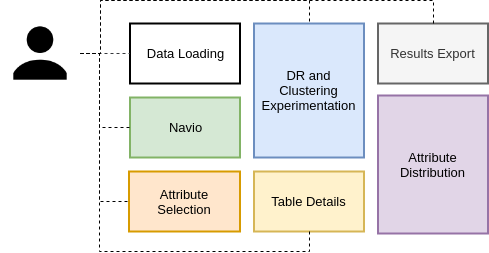
\includegraphics[width=0.7\textwidth]{MLExplore-components.png}
 \caption{MLExplore.js components and interaction possibilities for users.}
 \label{fig:mlexplore-components}
\end{figure}

In addition, the decision behind implementing the tool in a web-based environment with local ML computation using only JavaScript libraries for shareability, interactivity and on-device computation is inspired by Tensorflow.js \cite{Smilkov2019TensorFlow.js:Beyond}. These properties are important for domain-expert users because enable them to perform ML-based EDA without requiring complex infrastructure and easily share their work with colleagues and community in general. By the other hand, local computation also has the advantage of privacy preserving, because despite the tool is available on internet, the data remains in the browser. Currently, the ML community in JavaScript does not have the same level of development compared to other languages like Python and R, reason why alternatives for including ML algorithms in the tool are limited. Nevertheless, it is expected that this panorama continues evolving during the next years.

\section{Data Loading}
\label{section3.1}

In many cases, domain-expert users store data in local semi-structured files, principally when the size does not demand to invest resources to maintain TI infrastructures increasing the complexity of the project.
Currently. the tool supports loading datasets from a local path in CSV format and file size constraint depends on browser capabilities. In addition, as shown in Figure \ref{fig:load-dataset-component}, 4 low size datasets for trainees are available: (1) the Fisher's Iris \cite{FisherIris}, the Zoo dataset, the Breast Cancer dataset and the Heart Diseases dataset. All these datasets are available at UCI Machine Learning Repository \cite{Dua2017UCIRepository}.

\begin{figure}[ht]
 \centering
 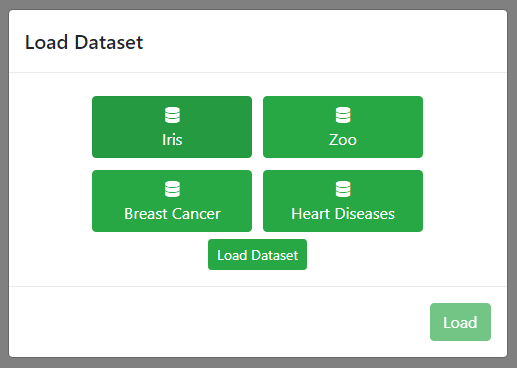
\includegraphics[width=0.5\textwidth]{load-dataset.png}
 \caption{Data Loading component.}
 \label{fig:load-dataset-component}
\end{figure}

\section{Data Exploration and Navigation (Navio)}
\label{section3.2}

The intention of using ML for exploring high-dimensional data does not imply that user should forget about descriptive techniques enabled also for gaining data understating. Distribution summarization, correlation analysis and outliers identification, among others, are generalized user tasks that always must be covered in any analytic process and considered in an Interactive ML tool as a element for \textbf{sample review}. Navio \cite{Guerra-Gomez2018Navio:Datasets} is an interactive web-based tool designed for achieving these kind of tasks but also for data navigation implementing three kinds of interactions: sorting, filtering a range and filtering by value. Because this tool is available as a JavaScript widget, the incorporation as a component requires a little effort and enables a more informed ML model usage. Figure \ref{fig:navio-component} shows the Navio component for the Breast Cancer dataset. 

\begin{figure}[ht]
 \centering
 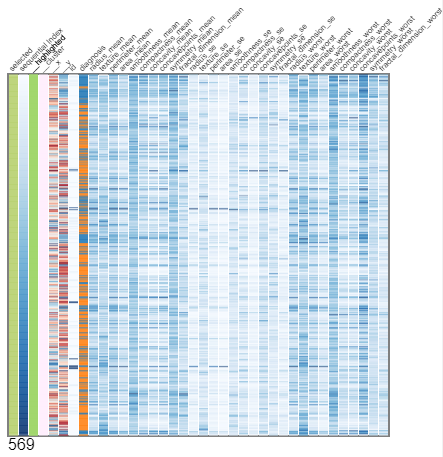
\includegraphics[width=0.5\textwidth]{navio.png}
 \caption{Data Exploration and Navigation (Navio) component.}
 \label{fig:navio-component}
\end{figure}

In addition, Navio component also includes three new attributes representing the results of the last trained models. This means, two new attributes for the embedding and other one for the clusters. In this way, user is enabled to extend the data exploration and navigation in the original space to, for instance, sort by embedding dimensions to discover correlations of them with data attributes or filter by a particular cluster. A fourth artificial attribute is used to retain highlighting actions performed by the user in the DR and Clustering Experimentation component.

\section{Attribute Selection}
\label{section3.3}

Attribute selection is an important stage in any ML process and it is a mechanism for providing \textbf{feedback assignment} when the domain-expert user decides if the presence of absence of a specific attribute can considerably affect the performance of a model. After the user load a dataset and performs an overview in Navio, all attributes are listed including an icon representing its type and a checkbox for attribute selection. Currently, the tool is able to identify two types of attributes: numerical and categorical. By default, all numerical attributes are selected meaning that these will be used for training the models. The reason behind this decision is related to the constraint of the models available in the tool for working only with numerical data. A Functionality for filter attributes by partial name matching, principally useful when there are a lot of similar attribute names, is also provided. Figure \ref{fig:attribute-selection-component} shows the Attribute Selection component for the Breast Cancer dataset.

\begin{figure}[ht]
 \centering
 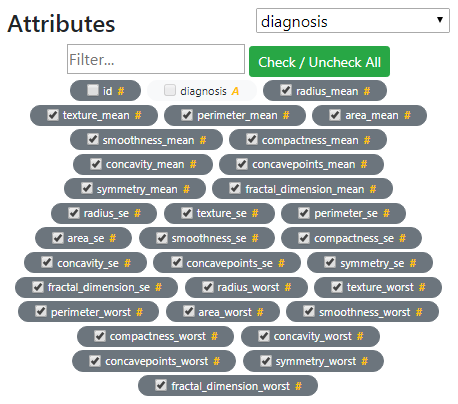
\includegraphics[width=0.5\textwidth]{attribute-selection.png}
 \caption{Attribute Selection component.}
 \label{fig:attribute-selection-component}
\end{figure}

In addition, the user can select the attribute for color encoding in the upper-right combobox affecting the DR and Clustering Experimentation and the Attribute Distribution components. If the attribute is categorical, a categorical color scheme is used but if the attribute is numerical, the color scheme selected by MLExplore.js is one sequential. Automatically, a categorical attribute with low cardinality is selected. A strategy for gaining interpretability about the results of the t-SNE algorithm is by selecting any numerical attribute and evidencing that higher values are concentrated in a zone of the embedding and lower values in a different. This principle is similar to the axis lines built in DimReader \cite{Faust2019DimReader:Projections} but not including additional elements which can make it more difficult to use these kind of tools.

\section{DR and Clustering Experimentation}
\label{section3.4}

The user is enabled to train in the browser two kind of DR and Clustering models for supporting the cluster-oriented EDA using the widely known t-SNE \cite{VanDerMaaten2008} and K-Means \cite{Lloyd1982LeastPCM} algorithms, and that currently have implementations in JavaScript \cite{Pezzotti2018LinearWeb},\cite{Asensio2018Ml-kmeans}. The result of t-SNE consist of two new dimensions or attributes being used for draw the a embedding (scatter plot) evidencing an overview of the data distribution. The result of K-Means is used for encode the color in the embedding and the Attribute Distribution component. For both models, the user can perform \textbf{feedback assignment} by modifying the hyper-parameters, re-train the models and visualize how the embedding and clusters changes in an iterative way. This is a way of \textbf{model inspection}. The t-SNE hyper-parameter ranges are based on \cite{Wattenberg2016HowEffectively}. Up to 10 number of clusters for K-Means training is allowed, this limit can be increased but losing readability because number of colors need to difference cluster or classes. MLExplore.js also enables user to scale attributes avoiding that models optimize paying more attention to attributes with high-range values. Figure \ref{fig:dr-and-clustering-experimentation-component} shows the DR and Clustering Experimentation component for the Breast Cancer dataset.

\begin{figure}[ht]
 \centering
 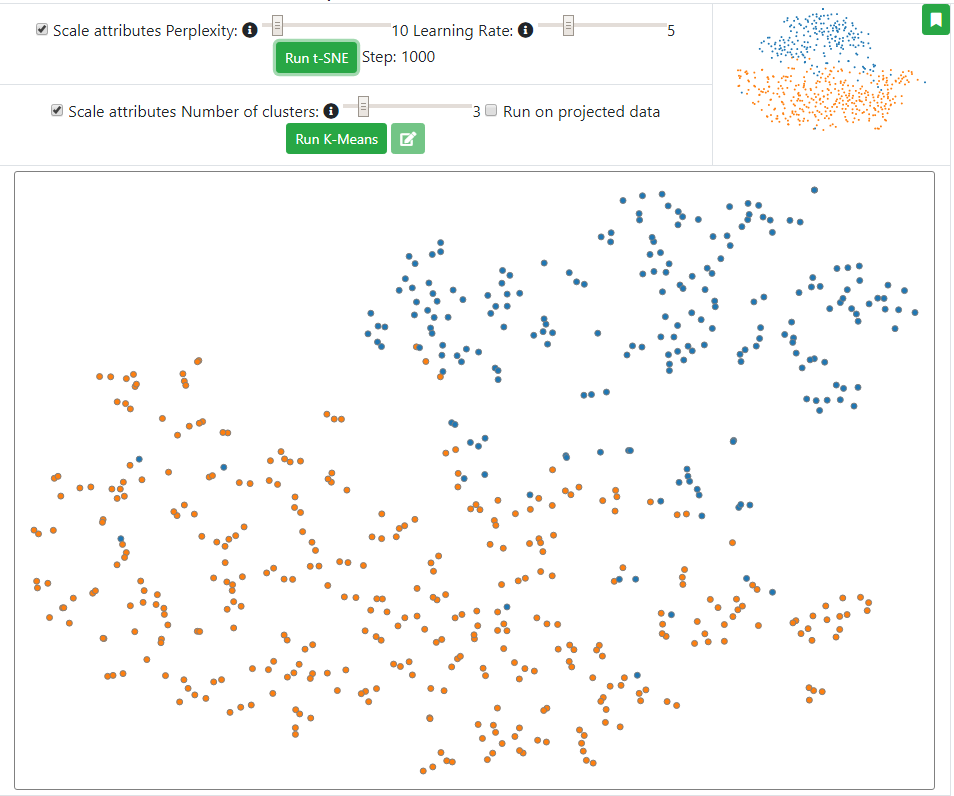
\includegraphics[width=0.7\textwidth]{dr-and-clustering-experimentation.png}
 \caption{DR and Clustering Experimentation component.}
 \label{fig:dr-and-clustering-experimentation-component}
\end{figure}

When finishing the training of a new model, additional changes to the embedding are produced: (1) Navio component is updated for including the results of the models, as explained in Section \ref{section3.2} and (2) Attribute Distribution component changes for evidencing the new clusters by color encoding. The user has the option to temporally save the current embedding and visualize the upper-right panel for model comparison. In addition, user is also enabled to change the cluster membership according to their judgment and highlight square regions of interest and visualize where some data instances are located in the Attribute Distribution component and how much their embedding distribution is differentiated from a previous experiment.

As a complementary \textbf{model inspection} strategy for interpretability, when user clicks a specific data instance, the embedding is updated to highlight the 20 nearest neighbors in terms of the Euclidean distance. This calculation can be useful to visually validate if, with those hyper-parameters, t-SNE is able to capture the similarity among data instances based in a more traditional metric that can be more easily understood by non-ML users. 

\section{Attribute Distribution}
\label{section3.5}

DR and Clustering models learn from similarity measures. If two data instances are close in the embedding or belongs to the same clusters, hopefully these instances will have similar attribute values. The purpose of this component is to evidence if this principle is fulfilled in a generalized way for \textbf{model inspection}, provide trust to user and advance in the insights extraction process. For each attribute used to train the models, a ticks chart or a scatter plot representing its distribution is displayed. The decision behind display a ticks chart or a scatter plot depends on the attribute currently used for color encoding. Figure \ref{fig:attribute-distribution-component} shows the Attribute Distribution component for the Breast Cancer dataset.

\begin{figure}[ht]
 \centering
 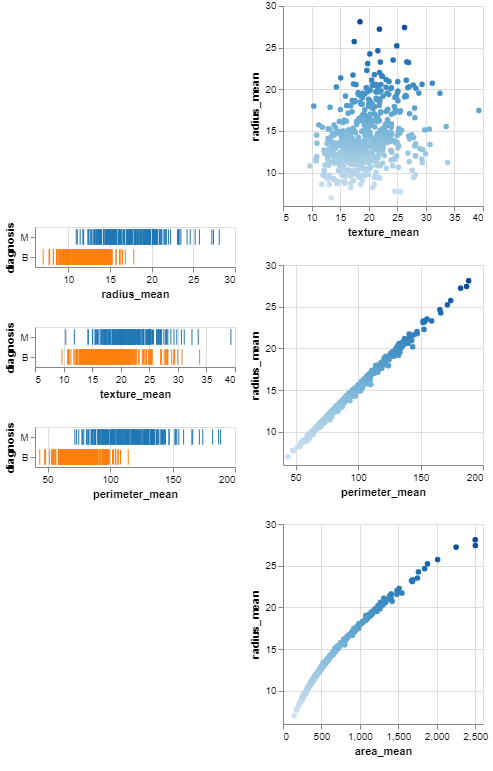
\includegraphics[width=0.4\textwidth]{attribute-distribution.png}
 \caption{Attribute Distribution component for categorical (left) and sequential (right) color encoding.}
 \label{fig:attribute-distribution-component}
\end{figure}

As mentioned before, this component is also affected by the DR and Clustering Experimentation component when user highlight a region of interest in the embedding. In the Attribute Distribution component, all data instances not included in the highlighting are opaqued. In this way, users are enabled to obtain details on demand.

\section{Table Details}
\label{section3.6}

Table Details component, a complementary \textbf{sample review} element, is included in MLExplore.js for enabling the data exploration in the most traditional way. This table is extended for searching data instances for by specific values, this functionality is useful in datasets like FIFA and SALURBAL in order to locate players, teams, positions or sub-cities, cities, countries, respectively. When user clicks a specific row, the embedding is updated to show the 20 nearest neighbors as previously explained in the DR and Clustering Experimentation component. Figure \ref{fig:table-details-component} shows this component for the Breast Cancer dataset.

\begin{figure}[ht]
 \centering
 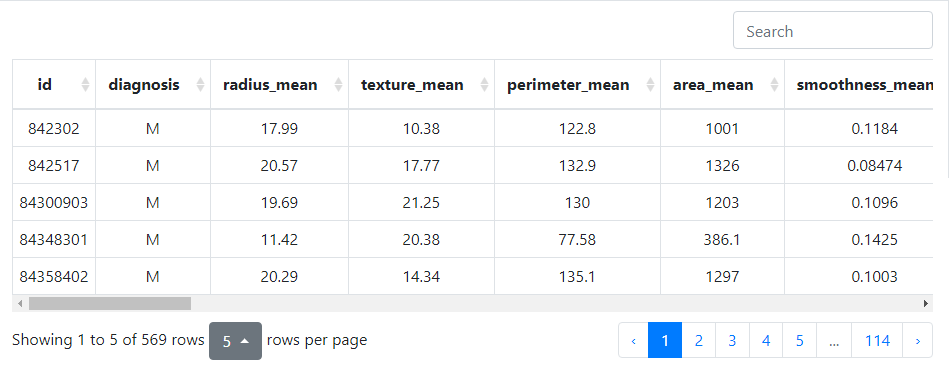
\includegraphics[width=0.9\textwidth]{table-details.png}
 \caption{Table Details component.}
 \label{fig:table-details-component}
\end{figure}

\section{Results Export}
\label{section3.7}

Finally, in any stage of the experimentation user is able to download the dataset in CSV format including all new artificial attributes (Navio selection, x-axis and y-axis embedding, clusters and highlighting) and a configuration file in JSON format. As shown in \ref{fig:results-export-component}, options provided when downloading the dataset include: download only model results, all attributes and model results and selected attributes and model results. The configuration file contains a list of the attributes, their identified type and which of these were used to train the models and encode the color during the last experimentation. Because the dataset is download in a widely known format, user can use it to continue with analysis process in almost any tool. Currently, this file only stores the hyper-parameters of the last trained models for the t-SNE and K-Means algorithms.

\begin{figure}[ht]
 \centering
 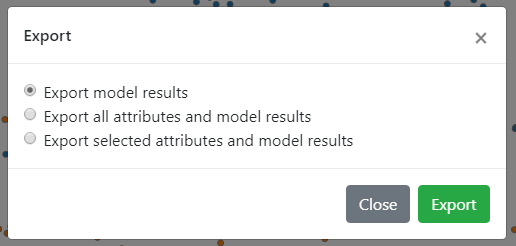
\includegraphics[width=0.5\textwidth]{results-export.png}
 \caption{Results Export component.}
 \label{fig:results-export-component}
\end{figure}